\documentclass[12pt,a4paper,utf8]{ctexart}
\usepackage{ctex,amsmath,amssymb,subfig,cite,graphicx,diagbox,fontspec,fancyhdr,geometry}
\usepackage[ntheorem]{empheq}
\usepackage{enumitem,fullpage,cleveref,cellspace,listings,color,framed}
\definecolor{gray}{rgb}{0.5,0.5,0.5}
\definecolor{dkgreen}{rgb}{.068,.578,.068}
\definecolor{dkpurple}{rgb}{.320,.064,.680}

%set Fortran styles
\lstset{
    frameround=tftf,
    language=Fortran,
    keywords={SELECT,PROGRAM,PRINT,STOP,END,WRITE,INTEGER,REAL,COMPLEX,CHARACTER,LOGICAL,READ,FORMAT,IMPLICIT,PARAMETER,DATA,EQUIVALENCE,TYPE,PAUSE,CONTINUE,CYCLE,EXIT,IF,SELECT,DO,ALLOCATE,DEALLOCATE,WHERE,FORALL,SUBROUTIHNE,CALL,RETURN,FUNCTION,COMMON,BLOCK DATA,SAVE,INTERFACE,CONTAIN,MODULE,USE,PUBLIC,PRIVATE,ENTRY,OPEN,INQUIRE,CLOSE,NAMELIST,POINTER,NULLFY,REWIND,BACKSPACE,ENDFILE
    },
    basicstyle=\footnotesize\ttfamily,
    numbers=left,
    numberstyle=\footnotesize,
    keywordstyle=\color{blue}\bfseries,
    commentstyle=\color{dkgreen},
    stringstyle=\color{dkpurple},
    backgroundcolor=\color{white},
    tabsize=2,
    showspaces=false,
    showstringspaces=false,
    breaklines=true,
    frame=trBL,
}
\CTEXsetup[format+={\raggedright}]{section}
\setlength{\parindent}{2em}
\geometry{
    textwidth=138mm,
    textheight=215mm,
    left=27mm,
    right=27mm,
    top=25.4mm,
    bottom=25.4mm,
    headheight=2.17cm,
    headsep=4mm,
    footskip=12mm,
    heightrounded,
}
\pagestyle{fancy}
\lhead{\textsl{2021秋-计算物理A}}
\chead{}
\rhead{\textsl{PB19020634-于浩然}}
\lfoot{}
\cfoot{\thepage}
\rfoot{}

\begin{document}
\begin{center}
    {\LARGE\textbf{计算物理作业十}}\\
    \textrm{于浩然}~~~~~~\textrm{PB19020634}~~~~~~\textrm{2021.11.07}
\end{center}

\section{作业题目}

Monte Carlo方法研究二维平面上荷电粒子在正弦外电场($\sim \sin \omega
t$)中的随机行走.推导速度自相关函数的表达式,它随时间的变化是怎样的行为?能否模拟得到该自相关函数的曲线?是的话与理论曲线进行比较,否的话讨论理由.

\section{算法简介}

\subsection{随机行走与抽样}

随机行走是运用Monte Carlo方法的一个模型. 设一个点从
$O$点出发,沿直线运动距离
$l$,此后转一个角度后再沿第二条直线运动距离$l$,上述过程重复$n$次后,求
点与初始点距离为$r + \textrm{d}r$的概率,这便是随机行走.

对于本题中的情况,我们不妨设电场对粒子作用力沿$x$轴方向,然后再将运动分解
为分别沿$x,y$轴的分运动,这样便把二维随机行走问题分解成了一个自由一维随机行走
和一个受周期性力约束的一维随机行走的叠加. 

我们先考虑$y$方向的自由随机行走. 不妨设粒子每步的步长$l_y=1$,且每一步向$y+,y-$方向运动
的概率均为$1/2$. 于是我们可对其进行抽样:
\begin{itemize}
    \item 抽取$[0,1]$上均匀分布的随机数$\eta_i$;
    \item 粒子沿$y$方向运动
        \begin{equation}
            \Delta y_i = 
            \begin{cases}
                -l_y,\quad 0 \leq \eta_i < 1/2 \\
                l_y, \quad 1/2 \leq \eta_i \leq 1
            \end{cases}
        \end{equation}
    \item $y_{i+1} = y_i + \Delta y_i$,重复上述过程$N$次.
\end{itemize}

接下来考虑$x$轴方向上受周期性电场力的随机行走.
此时粒子运动的方向将会受到电场力大小的调制,由于电场力大小的时变性,
在不同时间粒子向两个方向运动的概率将不同. 由于粒子受力大小与电场大小成正比,
我们不妨设外场$E \sim \sin \omega \tau$时粒子向两方向运动的概率如下:
\begin{equation}
    P(\Delta x = l_x) = 1/2 + k \sin \omega \tau, \quad 
    P(\Delta x = -l_x) = 1/2 - k \sin \omega \tau 
\end{equation}

其中$k$是速度影响移动方向概率的因子,由于概率值非负须满足约束关系
$k \leq 1/2$. 显见概率仍满足归一化. 在这里我们考虑最基本的RW模型,每一步
的步长相同,均为$l_x = 1$. 下面给出抽样方法:
\begin{itemize}
    \item 抽取$[0,1]$上均匀分布的随机数$\xi_i$;
    \item 粒子沿$x$方向运动
        \begin{equation}
            \Delta x_i(t) = 
            \begin{cases}
                - l_x, \quad 0 \leq \xi_i < 1/2 - k\sin \omega t \\
                l_x, \quad 1/2 - k \sin \omega t \leq \xi_i \leq 1 \\
            \end{cases}
        \end{equation}
    \item $x_{i+1} = x_i + \Delta x_i$,重复上述过程$N$次.
\end{itemize}

综上便可得出粒子随机行走任意时间后的坐标$(x_N,y_N)$.
\subsection{速度自相关函数}

自相关可以体现函数和自身的相关性. 
本题中考虑的速度为二维矢量,不妨设速度自相关函数为:
\begin{equation}
    C(t) = \langle \vec{v}(t) \cdot 
    \vec{v}(t_0) \rangle
\end{equation}

上面的$ \langle \cdot  \rangle $代表对大量粒子取平均得到的
期望值.
下面我们推导任意时刻的自相关函数:

不妨设粒子每步之间的时间间隔为单位时间,于是可以表示出粒子速度
\begin{equation}
    \vec{v}(t) \equiv \vec{v}_i = \vec{r}_{i+1} - \vec{r}_i = \Delta \vec{r}_i
    = \vec{e}_x \Delta x_i  + \vec{e}_y \Delta y_i
\end{equation}

下面的$p$指取相应值的概率,由(1)(3)式,
考察$ \vec{v}(t) \cdot\vec{v}(t_0)  $的取值与概率.
\begin{equation}
    v_y(t) v_y(t_0) = 
    \begin{cases}
        1, \quad (p=1/2) \\
        -1, \quad(p=1/2)
    \end{cases}
\end{equation}
\begin{equation}
    v_x(t) v_x(t_0) = 
    \begin{cases}
        1, \quad (p=1/2 + 2k^2 \sin \omega t_0\sin \omega t)\\
        -1, \quad (p=1/2 - 2k^2\sin \omega t_0\sin\omega t)
    \end{cases}
\end{equation}

可得
\begin{equation}
    \langle \vec{v}(t) \cdot \vec{v}(t_0)   \rangle = 4k^2 \sin \omega t_0
    \sin \omega t
\end{equation}

\section{编程实现}

使用FORTRAN90进行编程实现. 程序中将子程序 \texttt{Generator}写在模块
\texttt{RW}内,通过在主程序中调用 \texttt{Generator}实现不同参数的偏压
随机行走生成. 

按照理论推导预测,速度自相关函数应为周期函数,故步数选择不必多,在程序中取
200步,对$10^5$个粒子取平均. 其他参数分别选择为:
\begin{itemize}
    \item $\omega = 0.3,k = 0.5, t_0 = 30$
    \item $\omega = 0.5,k = 0.2, t_0 = 2$
    \item $\omega = 0.15,k = 0.15, t_0 = 50$
\end{itemize}

导出数据用python绘制图像,与理论曲线进行比较,结果展示在后面. 

\section{计算结果}

将上述3种参数条件下模拟得到的速度自相关函数曲线图展示如下:
\begin{figure}[htpb]
    \centering
    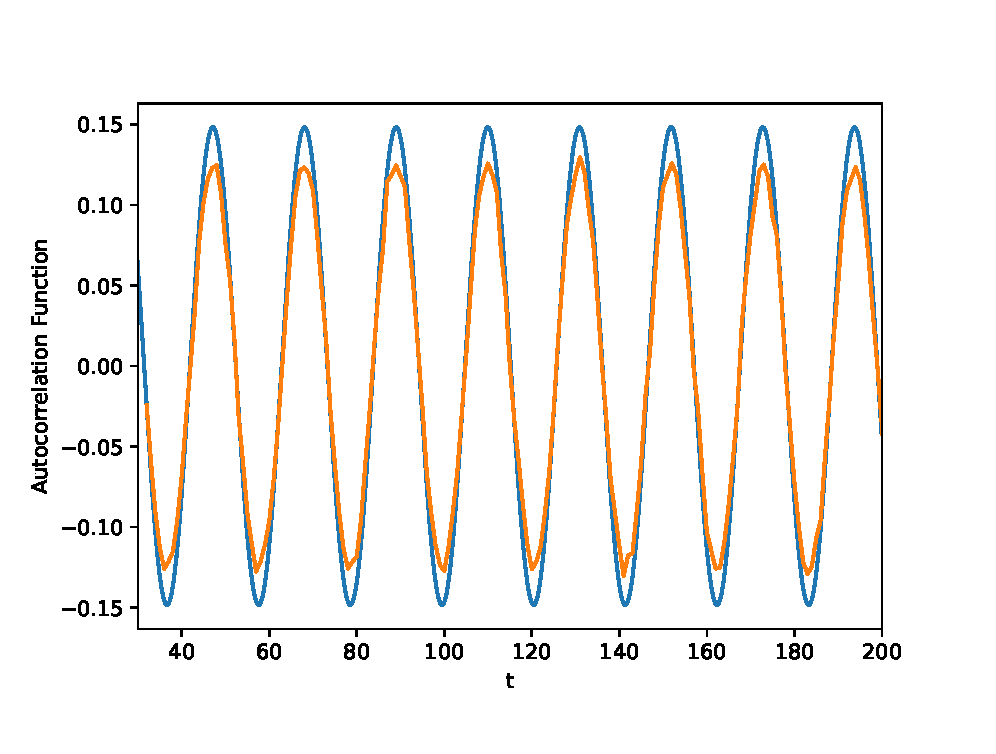
\includegraphics[width=0.8\textwidth]{fig1.eps}
    \caption{$\omega = 0.3,k = 0.5, t_0 = 30$下速度自相关函数曲线}
\end{figure}
\begin{figure}[htp]
    \centering
    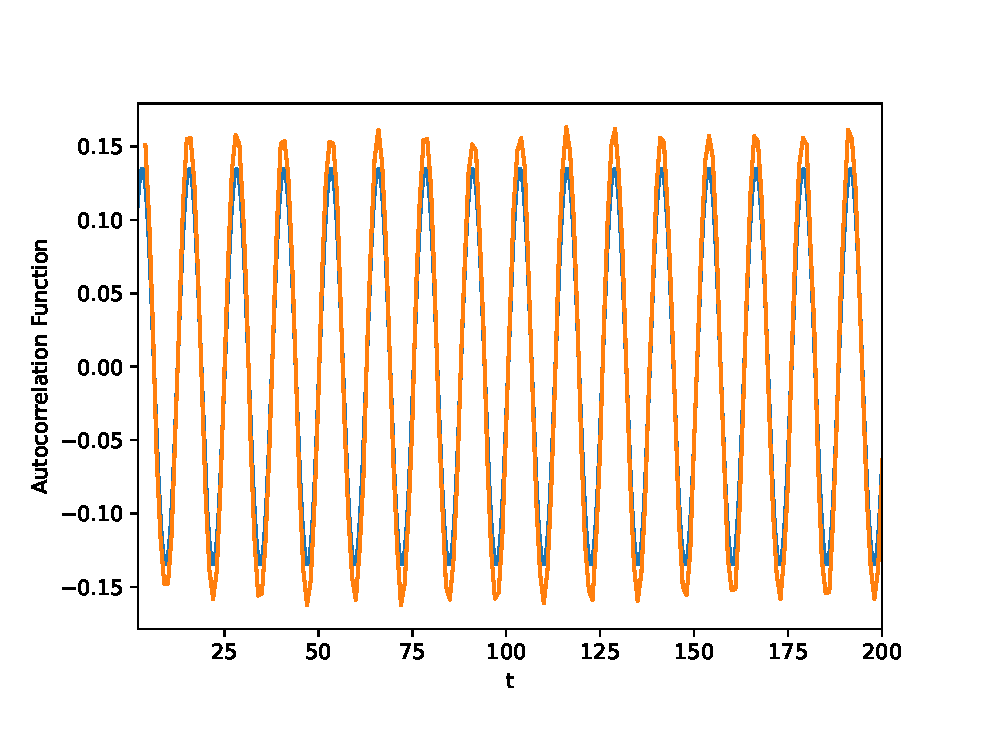
\includegraphics[width=0.8\textwidth]{fig2.eps}
    \caption{$\omega = 0.5,k = 0.2, t_0 = 2$下速度自相关函数曲线}
\end{figure}
\begin{figure}[htp]
    \centering
    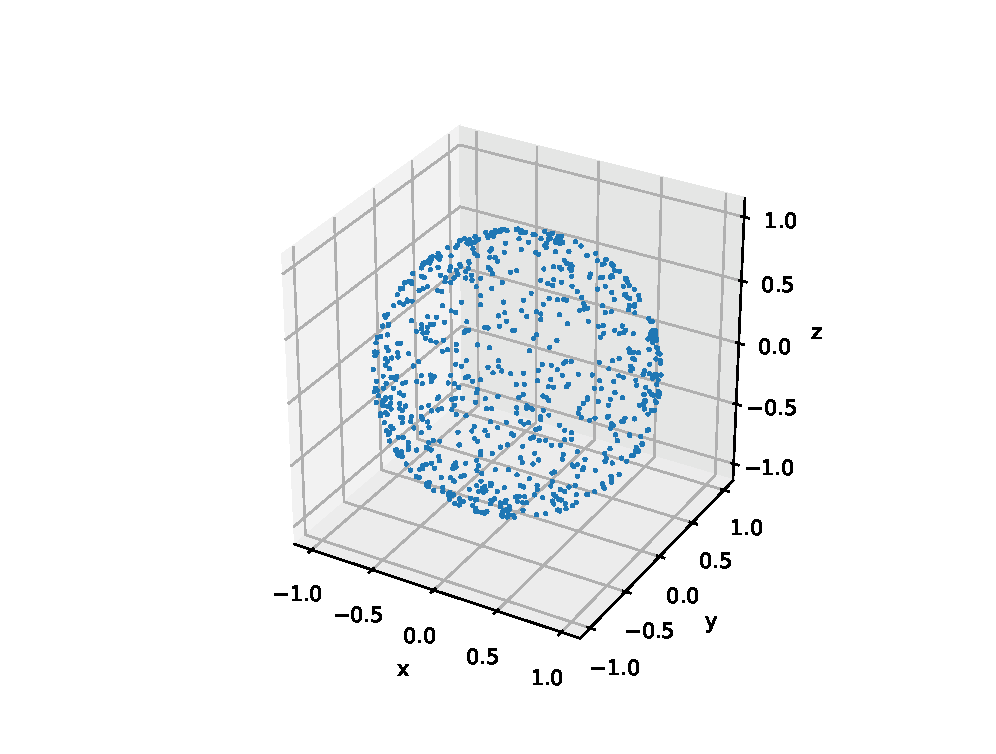
\includegraphics[width=0.8\textwidth]{fig3.eps}
    \caption{$\omega = 0.15,k = 0.15, t_0 = 50$下速度自相关函数曲线}
\end{figure}

\newpage
从图像中显然可看出,模拟得到的自相关函数呈现明显的周期性,且其周期值依赖于
$\omega$值,和理论符合的很好. 振幅和理论值存在一定差别,但仅限于在幅值最大时
比理论值稍大一点. 总的来说,模拟得到的自相关函数曲线与理论预测值符合得十分理想. 

\section{结论}

本题实现了偏压随机行走的生成,预言并验证了其速度自相关函数的具体形式,
即在周期性外力作用下的粒子的速度自相关函数将呈现和周期性外力相似的周期. 

\section{源代码}

FORTRAN90程序展示如下:
\begin{framed}
\begin{lstlisting}[language=Fortran]
MODULE RW
IMPLICIT NONE   
CONTAINS
SUBROUTINE Generator(particles, steps, omega, k, t0, filename) !随机行走生成器子程序
    INTEGER(KIND=4), INTENT(IN) :: particles, steps, t0
    CHARACTER(LEN=*), INTENT(IN) :: filename
    REAL(KIND=4), INTENT(IN) :: omega, k
    INTEGER(KIND=4) :: i, j, v(steps, particles, 2), &
        vdotproduct(2:steps, particles)
    REAL(KIND=8) :: seed, dat(steps * particles * 2), C(2:steps)
    
    PRINT *, 'Running...Please wait'
    CALL RANDOM_NUMBER(seed) !用FORTRAN自带的随机数生成器生成16807生成器的种子
    CALL Schrage(2 * particles * steps, int(2147483647 * seed), 'rand.dat')
    OPEN (1, file='rand.dat')
    READ (1, *) dat
    CLOSE (1)
    DO i = 1, steps 
        DO j = 1, particles
            !对速度y分量抽样
            IF(dat(2 * i * j) < 0.5) THEN
                v(i, j, 2) = -1
            ELSE
                v(i, j, 2) = 1
            END IF
            !对速度x分量抽样
            IF(dat(2 * i * j - 1) < 0.5 - k * SIN(omega * (i + t0))) THEN
                v(i, j, 1) = -1
            ELSE
                v(i, j, 1) = 1
            END IF
        END DO
    END DO
    DO i = 2, steps
        DO j = 1, particles
        vdotproduct(i, j) = DOT_PRODUCT(v(i, j, :), v(1, j, :))
        END DO
        !对多个粒子求点积的期望值,即为自相关函数值
        C = real(SUM(vdotproduct, DIM=2)) / particles 
    END DO
    OPEN (1, file=filename)
    WRITE (1, *) C !将速度自相关函数值写入文件
    CLOSE (1)
    PRINT *, 'Finished!'
END SUBROUTINE Generator
END MODULE RW

SUBROUTINE Schrage(num, z0, filename) !Schrage随机数生成器子程序
    IMPLICIT NONE
    INTEGER(KIND=4) :: N = 1, num
    INTEGER :: m = 2147483647, a = 16807, q = 127773, r = 2836, In(num), z0
    REAL(KIND=8) :: z(num)
    CHARACTER(LEN=8) :: filename
    In(1) = z0 !将传入值z0作为种子
    z(1) = REAL(In(1))/m
    DO N = 1, num - 1
        In(N + 1) = a * MOD(In(N), q) - r * INT(In(N) / q)
        IF (In(N + 1) < 0) THEN !若值小于零,按Schrage方法加m
            In(N + 1) = In(N + 1) + m
        END IF
        z(N + 1) = REAL(In(N + 1))/m !得到第N+1个随机数
    END DO
    OPEN (1, file=trim(filename)) !每次运行子程序按照传入参数filename生成数据文件
    DO N = 1, num !将随机数按行存入文件
        WRITE (1, *) z(N)
    END DO
    CLOSE (1)
END SUBROUTINE Schrage

PROGRAM MAIN
    USE RW
    CALL Generator(100000, 200, 0.3, 0.5, 30, 'scor1.dat')
    CALL Generator(100000, 200, 0.5, 0.2, 2, 'scor2.dat')
    CALL Generator(100000, 200, 0.15, 0.3, 50, 'scor3.dat')
END PROGRAM MAIN
\end{lstlisting}
\end{framed}

python绘图脚本展示如下:
\begin{framed}
\begin{lstlisting}[language=python]
import numpy as np
import matplotlib.pyplot as plt
import math

plt.rcParams['savefig.dpi'] = 300
plt.rcParams['figure.dpi'] = 300

t1 = 30
omega1 = 0.3
k1 = 0.3
y = np.loadtxt('scor1.dat')
x = np.arange(t1 + 2, t1 + 2 + np.size(y))
x1 = np.arange(0, 200, 0.1)
y1 = 4 * pow(k1, 2) * np.sin(omega1 * x1) * np.sin(omega1 * t1)
plt.xlim(t1, 200)
plt.xlabel('t')
plt.ylabel('Autocorrelation Function')
plt.subplots_adjust(bottom=0.15)
plt.plot(x1, y1)
plt.plot(x, y)
plt.savefig('fig1.eps')
plt.show()

t2 = 2
omega2 = 0.5
k2 = 0.2
plt.xlim(t2, 200)
y = np.loadtxt('scor2.dat')
x = np.arange(t2 + 2, t2 + 2 + np.size(y))
x2 = np.arange(0, 200, 0.1)
y2 = 4 * pow(k2, 2) * np.sin(omega2 * t2) * np.sin(omega2 * x2)
plt.xlabel('t')
plt.ylabel('Autocorrelation Function')
plt.subplots_adjust(bottom=0.15)
plt.plot(x2, y2)
plt.plot(x, y)
plt.savefig('fig2.eps')
plt.show()

t3 = 50
omega3 = 0.15
k3 = 0.3
plt.xlim(t3, 200)
y = np.loadtxt('scor3.dat')
x = np.arange(t3 + 2, t3 + 2 + np.size(y))
x3 = np.arange(0, 200, 0.1)
y3 = 4 * pow(k3, 2) * np.sin(omega3 * t3) * np.sin(omega3 * x3)
plt.xlabel('t')
plt.ylabel('Autocorrelation Function')
plt.subplots_adjust(bottom=0.15)
plt.plot(x3, y3)
plt.plot(x, y)
plt.savefig('fig3.eps')
plt.show()
\end{lstlisting}
\end{framed}
\end{document}

